\documentclass{article}

\usepackage[utf8]{inputenc}
\usepackage{graphicx}
\usepackage{caption}
\usepackage{listings}
\usepackage{lastpage}

\usepackage{hyperref}
\urlstyle{same}

\usepackage[export]{adjustbox} %center

% pakiety do języka polskiego
\usepackage[T1]{fontenc}
\usepackage[polish]{babel}
\usepackage[utf8]{inputenc}

\usepackage{indentfirst} % wcięcia

\captionsetup[figure]{name={caption}}

\title {Specyfikacja Implementacyjna Projektu ,,Optymalizacja Dostaw Szczepionek''} 
\author{Bartosz Zakrzewski}
\date{Data utworzenia 18.11.2020 \\ Data ostatniej modyfikacji 19.11.2020}

% Nagłówki na każdej stronie:
\usepackage{fancyhdr}
\pagestyle{fancy}
\fancyhf{}
\rhead{Bartosz Zakrzewski}
\lhead{Specyfikacja Impl. ,,Optymalizacja Dostaw Szczepionek''}
\rfoot{Strona \thepage \hspace{1pt} z \pageref{LastPage}}

\begin{document}
\maketitle
\thispagestyle{empty}

\clearpage
\tableofcontents
\thispagestyle{empty}

\clearpage

\section{Cel Projektu}
Celem projektu jest napisanie programu, który sprawi, że apteki kupią takie ilości szczepionek, od różnych producentów, za poszczególne ceny tak, że łączny koszt za wszystkie szczepionki będzie najmniejszy.

\section{Uruchomienie programu}

Aby program mógł wykonać obliczenia, należy dostarczyć do niego plik wejściowy poprawnie sformatowany i zawierający poprawne wartości.
\\

\par Jeżeli błąd wystąpi, program wypisze pierwszy napotkany błąd na konsolę i do pliku o nazwie ,,error.txt''. W przeciwnym razie użytkownik otrzyma plik wyjściowy o nazwie ,,optymalizacja.txt''.
Aby użytkownik mógł odnaleźć błąd w pliku wejściowym, program poinformuje, w jakiej linii znalazł go i jakiego rodzaju to był błąd.
\\ 
\par Uruchomienie następuje za pomocą java -jar:

\begin{lstlisting}
java -jar Optymalizacja.jar nazwa_pliku_wejsciowego.txt
\end{lstlisting}

\section{Środowisko pracy}
Program będzie implementowany na jednym komputerze przez jedną osobę.

\begin{itemize}
    \item System operacyjny - Windows 10
    \item IDE - Intellij IDEA 2020.2.3 Community Edition
    \item Java 14 (JDK 14)
    \item JUnit 4.13
    \item System kontroli wersji git, repozytorium umieszczone na platformie ISOD
\end{itemize}

\clearpage

\section{Zasady wersjonowania i językowe}
\begin{itemize}
    \item Commity będą po angielsku.
    \item Kod będzie pisany w języku angielskim.
    \item Gałęzie będą miały nazwę zaczynającą się od numeru porządkującego i słowa będą oddzielone znakiem ,,\_'' np. 04\_Find\_minimal\_difference.
    \item Odstępstwa od języka angielskiego mogą występować, gdy znaczenie w języku polskim jest unikalne: np. nazwy specyfikacji: gałąź o nazwie 01\_Specyfikacja\_Funkcjonalna.
    \item Jeżeli posługiwanie się językiem polskim ułatwi implementację, to można go użyć, np. używanie nazwy Apteka zamiast Pharmacy.
    \item Commity mogą zostać otagowane, jeżeli zajdzie taka potrzeba.
\end{itemize}

\section{Analiza pliku wejściowego i wykrycie algorytmu}
Wykrycie jak powinien działać algorytm odbędzie na podstawie analizy poniższego przykładu.

\begin{figure} [hbt!]
    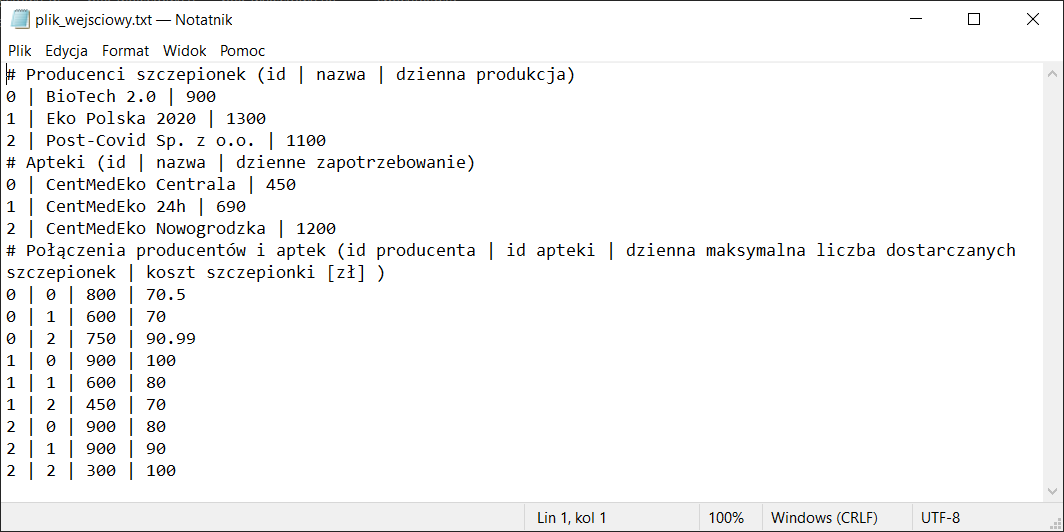
\includegraphics[width=18cm,center]{images/plik_wejsciowy.PNG}
    \captionof{figure}{Plik wejściowy}
\end{figure}

\clearpage

Najpierw zmienimy plik wejściowy w celu wizualizacji zależności między dzienną maksymalną liczbą dostarczanych szczepionek a dziennym zapotrzebowaniem.

\begin{figure} [hbt!]
    \includegraphics[width=16cm,center]{images/plik_wejsciowy_według_aptek.PNG}
    \captionof{figure}{Plik wejściowy posortowany według aptek}
\end{figure}

\clearpage

\subsection{Krok 1. Znalezienie ,,szczególnych'' połączeń aptek}
Znalezienie takiej apteki, że ma ona ma wyższe zapotrzebowanie niż suma dziennych maksymalnych liczb dostarczanych szczepionek dowolnych n-1 połączeń (n - liczba producentów). 
\\ 
\par Zobaczmy dla przykładu: \\
Dla Apteki o Id=2 należy zakupić minimum 450 szczepionek od producenta o Id=0, ponieważ nawet kupując od wszystkich innych producentów, nie zapełnimy dziennego zapotrzebowania.

\[450+300=750 = 1200-450 \]

\begin{figure} [hbt!]
    \includegraphics[width=16cm,center]{images/plik_wejsciowy_według_aptek_zaznaczone.PNG}
    \captionof{figure}{Na pewno musimy zakupić 450 sztuk w połączeniu 0 | 2}
\end{figure}

\clearpage
\subsection{Krok 2. Posortowanie połączeń poszczególnych aptek}
Następnie sortujemy połączenia poszczególnych aptek w zależności od kosztu szczepionki

\begin{figure} [hbt!]
    \includegraphics[width=16cm,center]{images/plik_wejsciowy_według_aptek_posortowany.PNG}
    \captionof{figure}{Połączenia według aptek posortowane}
\end{figure}

\clearpage

\subsection{Krok 3. Kupowanie szczepionek}
Zaczynamy od apteki, która ma największą różnicę między aktualną wartością najmniejszą i następną z kolei ze względu na cenę, kupujemy maksymalną ilość szczepionek za najniższą cenę, zwracając uwagę na dzienną produkcję i dzienną maksymalną liczbę dostarczanych szczepionek. Powtarzamy krok, aż dzienne zapotrzebowanie będzie uzupełnione.

\begin{figure} [hbt!]
    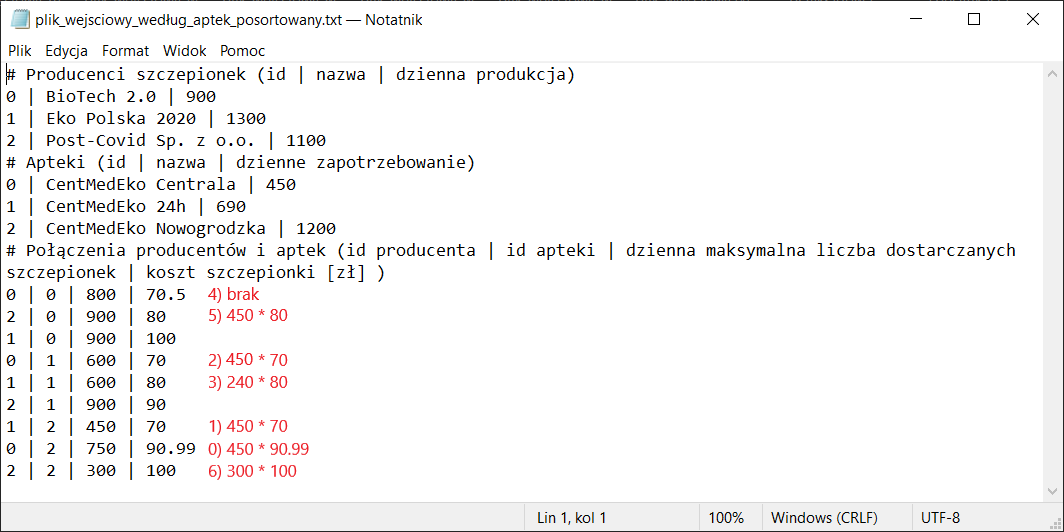
\includegraphics[width=16cm,center]{images/plik_wejsciowy_kolejnosc_kupowania.png}
    \captionof{figure}{Kolejność kupowania szczepionek}
\end{figure}

\clearpage

Ostateczna postać pliku wyjściowego:
\begin{figure} [hbt!]
    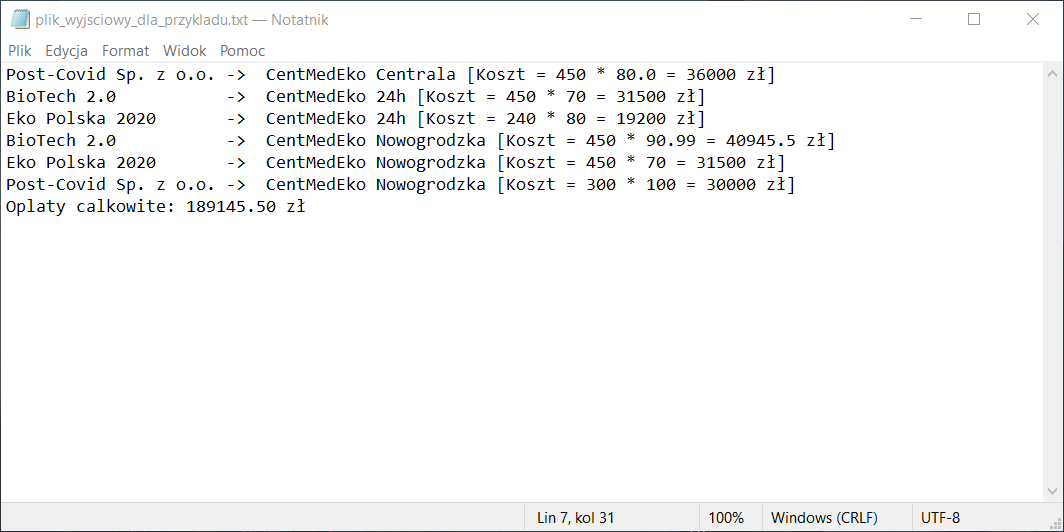
\includegraphics[width=16cm,center]{images/plik_wyjsciowy_dla_przykladu.PNG}
    \captionof{figure}{Plik wyjściowy minimalizacja}
\end{figure}

\clearpage

\section{Sprawdzenie ,,jakości'' minimalizacji}
Po zaimplementowaniu programu program będzie testowany z różnymi prawidłowymi danymi.
Kryterium jakości naszej minimalizacji będzie \textbf{błąd względny}.
\\ 
Gdyby kupić szczepionki nie zwracając uwagi na dzienną produkcję, wynik minimalizacji byłby inny i koszty byłyby najmniejsze z możliwych.
\\

Dla danego przykładu plik wyjściowy i koszty wyglądały by następująco:
\begin{figure} [hbt!]
    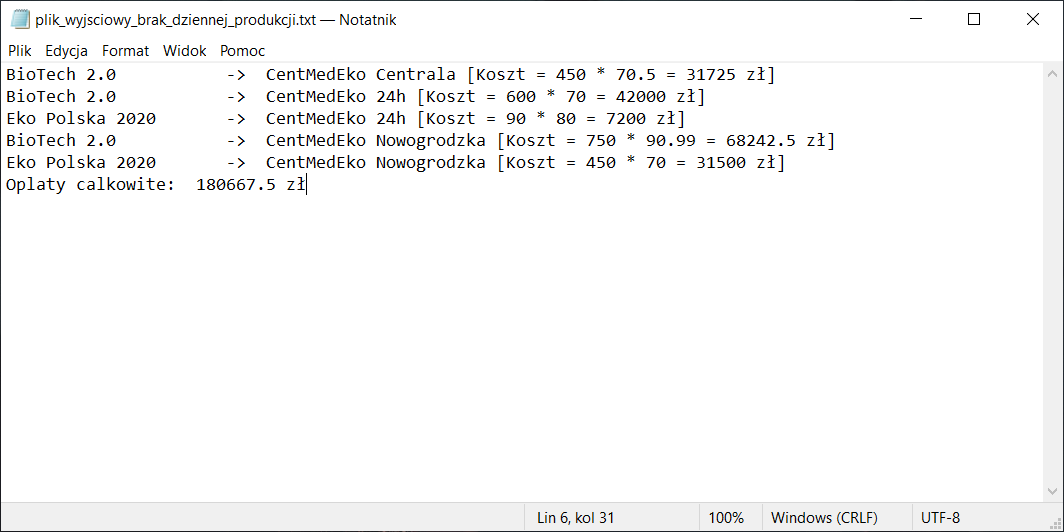
\includegraphics[width=16cm,center]{images/plik_wyjsciowy_brak_dziennej_produkcji.PNG}
    \captionof{figure}{Brak ograniczeń dziennej produkcji}
\end{figure}
\\
Dla przykładu błąd względny wynosi:
\[ (189145.50 - 180667.5) / 180667.5 = 0.0469 = 4.69\%\]

Dla innego rozłożenia ilości kupionych szczepionek i koszcie w przykładzie np. koszt całkowity = 190270.5 zł błąd względny wynosi:
\[ (190270.5 - 180667.5) / 180667.5 = 0.0532 = 5.32\%\]

Jeżeli błąd względny będzie wynosił więcej niż 10\% to użytkownik zostanie powiadomiony o tym że minimalizacja nie jest optymalna przez wyświetlenie na konsolę i do pliku ,,blad\_wzgledny.txt''

\section{Analiza algorytmu}
\subsection{Krok 0. Wczytanie poszczególnych wartości}
Wartości zostaną wczytane do obiektów klas ,,Producer'', ,,Pharmacy'', ,,Connection''. Znajdą się one w listach liniowych z pakietu java.util.ArrayList<E> (ArrayList<Producer> i ArrayList<Pharmacy>).
Natomiast Connections będą znajdowały się w wielu ArrayListach odpowiednich do każdej apteki, np. listOfConnectionsOfPharmacy0, listOfConnectionsOfPharmacy1, itd.

\subsection{Krok 1. Znalezienie ,,szczególnych'' połączeń aptek}
Aby odnaleźć szczególną aptekę, należy sprawdzić wszystkie kombinacje sum dziennych maksymalnych liczb dostarczonych szczepionek. Takich kombinacji dla naszego przykładu jest 3, a dla n producentów takich kombinacji jest:
\[ {n \choose n - 1} = n \]
Aby odnaleźć poszczególne kombinacje posłuże się algorytmem znalezionym na stronie: \\
\url{https://www.geeksforgeeks.org/print-all-possible-combinations-of-r-elements-in-a-given-array-of-size-n/}

\subsection{Krok 2. Posortowanie połączeń poszczególnych aptek}
Połączenia umieszczone w listach zostaną posortowane według kosztu szczepionki za pomocą sortowania szybkiego.
Złożoność w notacji dużego O - liniowo-logarytmiczna.

\subsection{Krok 3. Kupowanie szczepionek}
Aby sprawdzać dzienne zapotrzebowanie i dzienną produkcję należy przejść przez listy producentów i aptek, i zaktualizować poszczególne wartości.
Złożoność w notacji dużego O - liniowa.

\clearpage

\section{Źródła}

\begin{itemize}
    \item Opis problemu, przykładowy plik wejściowy i wyjściowy przygotował i umieścił na platformie ISOD mgr inż. Paweł Zawadzki
    \item Rysunki poglądowe zostały wykonane za pomocą programu Paint 3D
    \item Ten dokument został stworzony na stronie overleaf.com
\end{itemize}

\end{document}